
\documentclass{article}

% Language setting
% Replace `english' with e.g. `spanish' to change the document language
\usepackage[polish]{babel}
\usepackage{indentfirst} 

% Set page size and margins
% Replace `letterpaper' with `a4paper' for UK/EU standard size
\usepackage[a4paper,top=2cm,bottom=2cm,left=3cm,right=3cm,marginparwidth=1.75cm]{geometry}

% Useful packages
\usepackage{amsmath}
\usepackage{graphicx}
\usepackage{listings}
\usepackage{url}
\usepackage{xcolor}
\usepackage[colorlinks=true, allcolors=blue]{hyperref}

\definecolor{codegreen}{rgb}{0,0.6,0}
\definecolor{codegray}{rgb}{0.5,0.5,0.5}
\definecolor{codepurple}{rgb}{0.58,0,0.92}
\definecolor{backcolour}{rgb}{1,1,1}

\lstdefinestyle{mystyle}{
    backgroundcolor=\color{backcolour},   
    commentstyle=\color{codegreen},
    keywordstyle=\color{orange},
    numberstyle=\tiny\color{codegray},
    stringstyle=\color{codegreen},
    basicstyle=\ttfamily\footnotesize,
    breakatwhitespace=false,         
    breaklines=true,                 
    captionpos=b,                    
    keepspaces=true,                 
    numbers=left,                    
    numbersep=5pt,                  
    showspaces=false,                
    showstringspaces=false,
    showtabs=false,                  
    tabsize=2
}

\lstset{style=mystyle}

\title{Implementacja wskaźnika giełdowego MACD}
\author{Konrad Bryłowski, 188577}

\begin{document}
\maketitle

\section{Wstęp}

\subsection{Wskaźnik MACD}

Celem projektu była implementacja wskaźnika MACD. Wskaźnik MACD (moving average convergence/divergence - zbieżność/rozbieżność średniej kroczącej) jest jednym z najczęściej używanych wskaźników używanych do analizy technicznej danych giełdowych. Zaletami tego wskaźnika jest łatwa implementacja i interpretacja wyników. Jego główną wadą jest spóźniona informacja o potrzebie kupna i sprzedaży instrumentów kapitałowych, dlatego używa się go przede wszystkim do inwestycji długoterminowych.

Wskaźnik MACD opiera się na średniej kroczącej (EMA), to jest średniej ważonej, w której wartości bardziej odległe od obecnej wartości mają wykładniczo mniejszą wagę oraz pod uwagę brana jest określona liczba poprzednich wartości.

Wskaźnik składa się z dwóch linii - MACD oraz SIGNAL. Wartość linii MACD jest różnicą EMA wartości instrumentu z okresu 12 dni (okresów) (zwaną również szybką EMA) oraz 26 dni (zwaną wolną EMA) \cite{web:wiki} Natomiast wartość linii SIGNAL jest średnią kroczącą z wartości linii MACD z 9 dni. Sygnałem do zakupu albo sprzedaży jest przecięcie tych dwóch linii na wykresie.

\[\alpha = \frac{2}{N + 1}\]
\[EMA_N = \frac{\sum_{i = 0}^N p_i (1 - \alpha)^i}{\sum_{i = 0}^N(1-\alpha)^i}\]
gdzie $N$ jest liczbą okresów poprzedzających, a $p_i$ próbką sprzed $i$ dni.
\[MACD = EMA_{12} - EMA_{26}\]

\subsection{Dane wejściowe}

Jako dane wejściowe użyto amerykańskiego indeksu S\&P500 (SPX) w okresie 1000 cen zamknięcia (w USD) od 27 marca 2019. Dane pochodzą z zasobów \href{https://stooq.com/q/d/?s=^spx&c=0&d1=20190325&d2=20230315}{stooq.com}. Wykres cen zamknięcia w kolejnych dniach został przedstawiony na Rysunku \ref{fig:input_data}.

\begin{figure}[!b]
\centering
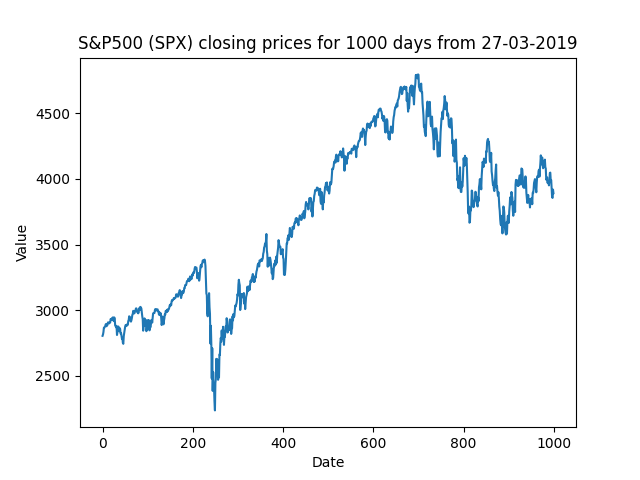
\includegraphics[width=0.85\textwidth]{input_data.png}
\caption{\label{fig:input_data}Dane wejściowe}
\end{figure}

\section{Implementacja}

Do implementacji wskaźnika użyto języka Python z modułami \texttt{matplotlib} do tworzenia wykresów, \texttt{pandas} do odczytania pliku w formacie csv z danymi wejściowymi oraz \texttt{numpy} do obliczeń.

\subsection{Linie MACD oraz SIGNAL}

Przy stosowaniu wzoru na wartość linii MACD oraz SIGNAL przez pierwsze okresy przyjęto zmniejszoną wartość $N$, przez co wyniki w pierwszych dniach mogą być niedokładne. Algorytm został podzielony na funkcje liczące EMA dla zadanego okresu, liczącą MACD, wyznaczającą momenty kupna/sprzedaży oraz prezentujące wyniki. Każda funkcja zawiera komentarz w formacie \texttt{docstring}, który w listingach zostanie pominięty.

\begin{lstlisting}[language=Python, caption=Funkcja obliczająca MACD, captionpos=b]
def calculate_macd(path: str) -> tuple[pd.Series, pd.Series]:
    with open(path, 'r') as f:
        data = pd.read_csv(f)
        dates = data.loc[:, 'Date']
        closing_prices = data.loc[:, 'Close']
        signal = []
        macd = []
        for date, price in zip(dates, closing_prices):
            slow = calculate_slow_ema(date, dates, closing_prices)
            fast = calculate_fast_ema(date, dates, closing_prices)
            macd.append(fast - slow)
            if len(macd) < 9:
                signal.append(calculate_ema(dates[:len(macd)], \
                    pd.Series(macd)))
            else:
                signal.append(calculate_ema(dates[len(macd) - \
                    9:len(macd)], pd.Series(macd[len(macd) - \
                    9:len(macd)])))
        return pd.Series(macd), pd.Series(signal)
\end{lstlisting}

Funkcje \lstinline{calculate_slow_ema} oraz \lstinline{calculate_fast_ema} wyznaczają odpowiednie indeksy początkowe i końcowe przedziałów dla podanej daty i zwracają wynik funkcji \lstinline{calculate_ema} dla odpowiednich przedziałów danych.

\begin{lstlisting}[language=Python, caption=Funkcja obliczająca wartość $EMA_N$, captionpos=b]
def calculate_ema(dates: pd.Series, prices: pd.Series) -> float:
    N = len(dates) - 1
    alfa = 2 / (N + 1)
    numerator = 0
    denominator = 0
    for i in range(N):
        price = prices.iat[i]
        numerator += price * (1 - alfa) ** (N - i)
        denominator += (1 - alfa) ** (N - i)
    numerator += prices.iat[N]
    denominator += 1
    ema = numerator / denominator
    return ema
\end{lstlisting}

\subsection{Wyznaczanie punktów zakupu i sprzedaży instrumentu}

Aby wyznaczyć dni zakupu oraz sprzedaży akcji należy wyznaczyć punkty przecięcia obu linii. W przypadku przecięcia linii SIGNAL przez MACD od dołu jest to sygnał do kupna, w przeciwnym razie - do sprzedaży.

\begin{lstlisting}[language=Python, caption=Funkcja wyznczająca punkty przecięcia MACD i SIGNAL, captionpos=b]
def calculate_buy_sell(macd: pd.Series, signal: pd.Series) \
        -> tuple[pd.Series, pd.Series]:
    buy = [np.nan]  # don't buy on the first day
    sell = [np.nan]  # don't sell on the first day
    for i in range(1, len(macd)):
        if macd[i - 1] < signal[i - 1] and macd[i] >= signal[i]:
            # MACD crosses SIGNAL from below
            buy.append(macd[i])
            sell.append(np.nan)
        elif macd[i - 1] > signal[i - 1] and macd[i] <= signal[i]:
            # MACD crosses SIGNAL from above
            buy.append(np.nan)
            sell.append(macd[i])
        else:
            # no crossing
            buy.append(np.nan)
            sell.append(np.nan)
    return pd.Series(buy), pd.Series(sell)
\end{lstlisting}

\section{Wyniki}

\begin{figure}[h]
\centering
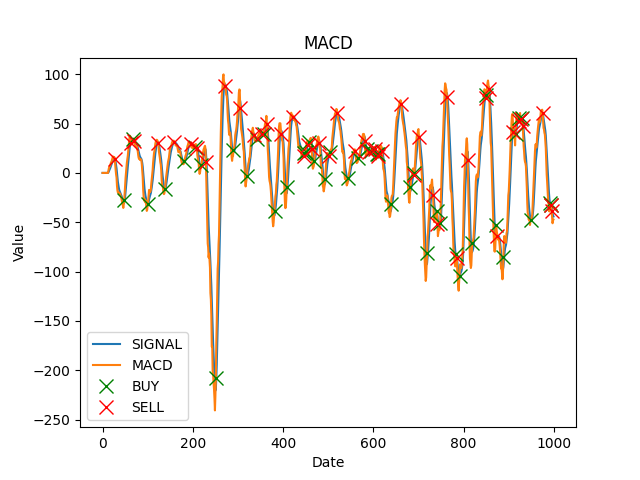
\includegraphics{macd.png}
\caption{\label{fig:macd}Wykres wskaźnika MACD}
\end{figure}

\begin{figure}[ht]
\centering
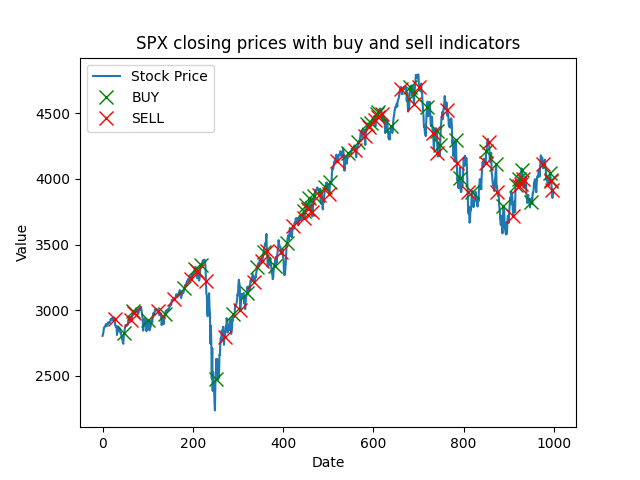
\includegraphics{stock_prices.png}
\caption{\label{fig:stock_prices}Momenty zakupu/sprzedaży wyznaczone za pomocą MACD naniesione na wykres cen}
\end{figure}

Analizując Rysunek \ref{fig:stock_prices} można zauważyć opóźnienie wyznaczonych za pomocą wskaźnika MACD momentów kupna oraz sprzedaży instrumentu względem najbardziej optymalnych. Za przykład może posłużyć duży spadek wartości instrumentu między 200 a 300 dniem (co przypada na początek lockdownów na świecie w 2020 r.) - w tym miejscu informacja o konieczności sprzedaży była opóźniona, co wywołało stratę w ujęciu krótkoterminowym. Również po zakończeniu tego spadku informacja o potrzebie kupna pojawiła się już po wzroście ceny z najkorzystniejszej, co obniżyło zysk. W następnych okresach w czasie trendu wzrostowego korzystniejsze byłoby przetrzymanie zamiast ciągłego sprzedawania i kupowania w większej cenie.

Jednak biorąc pod uwagę perspektywę długoterminową, w której pojedyncza gorsza lub spóźniona decyzja mają mniejsze znaczenie niż w ujęciu krótkoterminowym, wskaźnik MACD może okazać się przydatny. W praktyce, aby zapewnić lepszą efektywność, wprowadza się dodatkowe warunki do sygnałów kupna lub sprzedaży - na przykład sygnał kupna zostaje wygenerowany przy niedodatniej wartości linii MACD lub sygnał sprzedaży - gdy linia SIGNAL jest nierosnąca \cite{web:ing}.

\section{Ocena efektywności}

\subsection{Zastosowany algorytm}

\begin{lstlisting}[language=Python, caption=Algorytm symulujący zysk/stratę, captionpos=b]
def calculate_profit(prices: pd.Series, buy: pd.Series, sell: pd.Series, \
        initial_cash: float, initial_holdings: int) -> tuple[float, float]:
    value = 0
    holdings = initial_holdings
    cash = initial_cash
    for i in range(1, len(prices)):
        if not np.isnan(buy.iat[i]):
            if cash > 0:
                holdings += cash // prices.iat[i]
                cash -= holdings * prices.iat[i]
        elif not np.isnan(sell.iat[i]):
            if holdings > 0:
                cash += holdings * prices.iat[i]
                holdings = 0
        value = holdings * prices.iat[i]
    profit = value + cash - initial_cash - initial_holdings * prices.iat[0]
    return profit, value + cash
\end{lstlisting}

W momencie wystąpienia sygnału kupna inwestowane są wszystkie dostępne środki, a przy wystąpieniu sygnału sprzedaży sprzedawane są wszystkie jednostki instrumentu. Funkcja zwraca ostateczny zysk (a w przypadku straty wartość ujemną) oraz sumę ostatecznej wartości posiadanych jednostek oraz wolnych środków. Algorytm zakłada brak możliwości posiadania ułamkowych części jednostek.

\subsection{Wynik symulacji}

Przy początkowym kapitale wynoszącym 1000 jednostek indeksu S\&P500 oraz \$0 wolnych środków (wartość 2.805 mln dolarów), wartość końcowa wyniosła 3.802 mln dol., to jest około 997 tys. dolarów zysku.

Gdyby przez cały okres trzymać początkowe 1000 jednostek indeksu SPX ostateczna wartość wyniosłaby 3.891 mln dolarów.

\subsection{Wnioski}

Zastosowany algorytm nie podejmuje decyzji czy podjąć ryzyko wstrzymania się w całości lub w części z zakupem lub sprzedażą jednostek instrumentu, ale jedynie reaguje na sygnały wynikające z MACD. Nie są brane pod uwagę takie czynniki jak specyfika danego instrumentu (np. w przypadku SPX to, że indeks ten zawsze charakteryzował się wzrostem wartości w dłuższych okresach). Minimalizuje on konieczność podejmowania decyzji dotyczących ryzyka przez użytkownika, jednak nie jest nieomylny, ponieważ nie ma dostępu do przyszłych cen, a jedynie je przewiduje na podstawie danych historycznych.

Mimo swoich wad algorytm ten osiągnął zysk w symulacji, ponieważ błędne, przedwczesne lub spóźnione decyzje zostały przeważone przez długoterminowy zysk. Z tego względu nie nadaje się on do krótkoterminowych inwestycji.

\bibliographystyle{plain}
\bibliography{sample}

\end{document}